\documentclass[onecolumn, 12pt]{IEEEConf}
\usepackage{xr}
\usepackage{zref}
\usepackage{graphicx}
\usepackage{float}
\usepackage[export]{adjustbox}
\usepackage{setspace}
\usepackage{url}


\input{"C:/Users/Klaethis/Documents/Latex Templates/CodeFormat.tex"}
\input{"C:/Users/Klaethis/Documents/Latex Templates/MathFormat.tex"}


\renewcommand{\thesection}{\Roman{section}}
\renewcommand{\thesubsection}{\Alph{subsection}}
\renewcommand{\thesubsubsection}{\roman{subsubsection}}


\title{Final Project Report}
\author{Mike Zimmerman \\ ECE-3780-001 \\ Communications Systems}
\date{\today}


\begin{document}
    \maketitle
    \doublespacing
    \section{Introduction}
        The purpose of this project was to demonstrate a wireless communication system.
        The system chosen for this project was the Wi-Fi\footnote{Wi-Fi is a registered trademark of the Wi-Fi alliance.} wireless communication protocol.
        This protocol was selected for its ubiquity and ease of use.
        In order to implement our communication, a microcontroller (MCU), was selected that natively supported Wi-Fi.

        In order to show that wireless communication was possible, two different systems were created.
        One as the server, and another as the client.
        The server has an environment sensor attached, and would send the data to connected clients.
        The client would detect the server device, connect, gather the transmitted data, and display the values on a screen.
        As a secondary client, the server would also produce a simple webpage that a computer could display.

    \section{Wi-Fi Background}
        The chosen wireless communication for this project was Wi-Fi.
        It was created as it is known today by the Wi-Fi Alliance in september 1998, and is now the most popular wireless communication protocol.\cite{Wi-Fi_History}
        It uses the IEEE 802.11 standard. 

        Wi-Fi uses radio waves in the 2.4 GHz or 5 GHz frequencies to transmit and receive digital data.
        These frequencies are in Ultra High, and Super High frequency bands.

    \section{ESP8266}
        Espressif is a semiconductor company based out of Shanghai China. \cite{About_Espressif}
        They create chip-sets for Wi-Fi, bluetooth, and Internet of Things (IoT) products.
        While they are a relatively new company, their accessability and price point has
        greatly aided in moving them to the forefront of the maker movement.

        A large factor to their popularity is the ESP8266 microcontroller.
        The ESP8266EX System On a Chip (SOC) was launched in May 2014.\cite{Espressif_Milestones}
        This was the chip behind the ESP-01 module.
        The ESP-01 module is a low-cost microcontroller designed to give another microcontroller an 
        easy way to connect to Wi-Fi.

        Many engineers realized the ESP8266EX was powerful enough to be the main processor for many applications,
        but the ESP-01 lacked a large amount of connected General Purpose Input Output (GPIO) pins.
        This was the driving force behind the development of other modules using the ESP8266EX that had larger
        numbers of connected GPIO pins.

    \section{Weather Station Project}
        The basic design of this project was to have an environment sensor,
        and a display unit.
        The display unit would need to be able to show the basic information
        being transmitted by the sensor unit.
        The sensor unit would also need to be able to handle multiple connections at once.

        For this setup, the sensor acting as a Wi-Fi access point, and as a basic web server
        made the development easy. The block diagram of the project can be seen in Figure~\ref{fig:BlockDiagram}.
        
        \begin{figure}
            \centering
            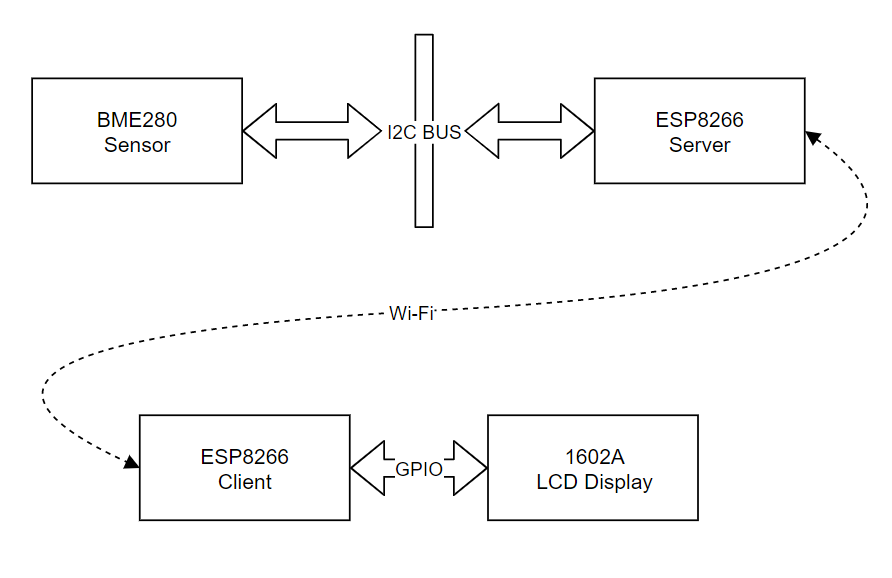
\includegraphics[max width=\textwidth,keepaspectratio,scale=.6]{images/BlockDiagram.png}
            \caption{\label{fig:BlockDiagram}Block diagram of the weather station project}
        \end{figure}

    \subsection{Sensor Development}
        The sensor unit was designed with an ESP8266 development board.
        This was connected to a BME-280 temperature, pressure, and humidity sensor via the
        Inter-Integrated-Circuit (I2C) protocol.
        The schematic for the circuit can be seen in Figure~\ref{fig:ServerSchematic}.
        
        \begin{figure}
            \centering
            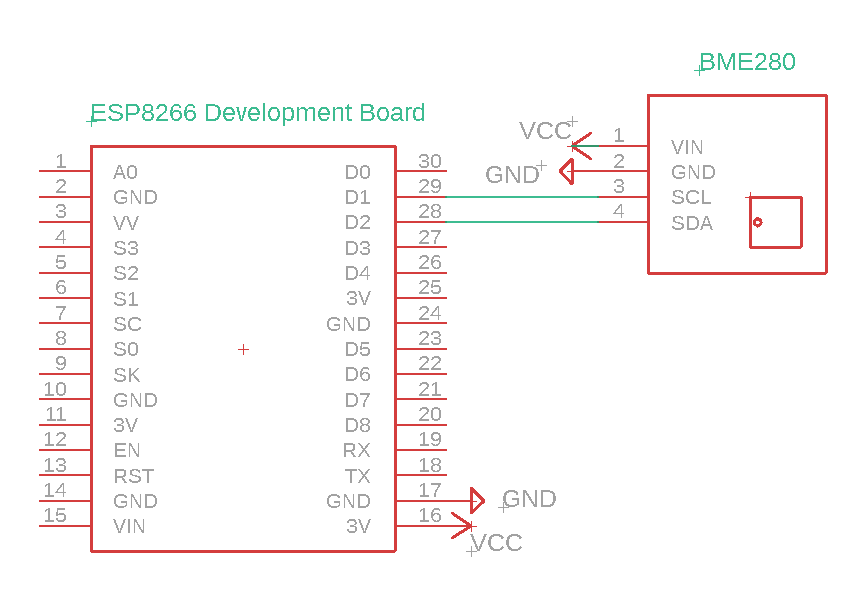
\includegraphics[max width=\textwidth,keepaspectratio,scale=.6]{images/ServerSchematic.png}
            \caption{\label{fig:ServerSchematic}Sensor schematic}
        \end{figure}

        The firmware development for the sensor was made simple by the use of pre-made libraries
        surrounding the use of the BME-280 sensor and Wi-Fi stack.

        The basic idea behind the sensor firmware was to set up a Wi-Fi access point, and wait for client connections.
        After a client would connect, it would then request a pre-determined URL for the current environment data.
        The sensor would then query the BME-280, format a return string, and transmit a reply to the client.

        The design of the senor could require that it be placed somewhere that is difficult to directly access.
        Due to this, it was prudent to implement an Over The Air (OTA) update system.
        This causes the microcontroller to withhold half of its program flash for an update to be copied.
        When an update is sent to the ESP8266, it copies the firmware to the second half of the flash.
        When the transmission is complete, it will then verify the firmware it has received, and then reboot.
        When the reboot is underway, it will then load the new firmware instead of the old firmware.

    \subsection{Display Development}
        The display circuit was also designed with an ESP8266 development board.
        It was connected to a 1602A 16x2 LCD display via GPIO pins.
        The schematic for the circuit can be seen in Figure~\ref{fig:ClientSchematic}.
        
        \begin{figure}
            \centering
            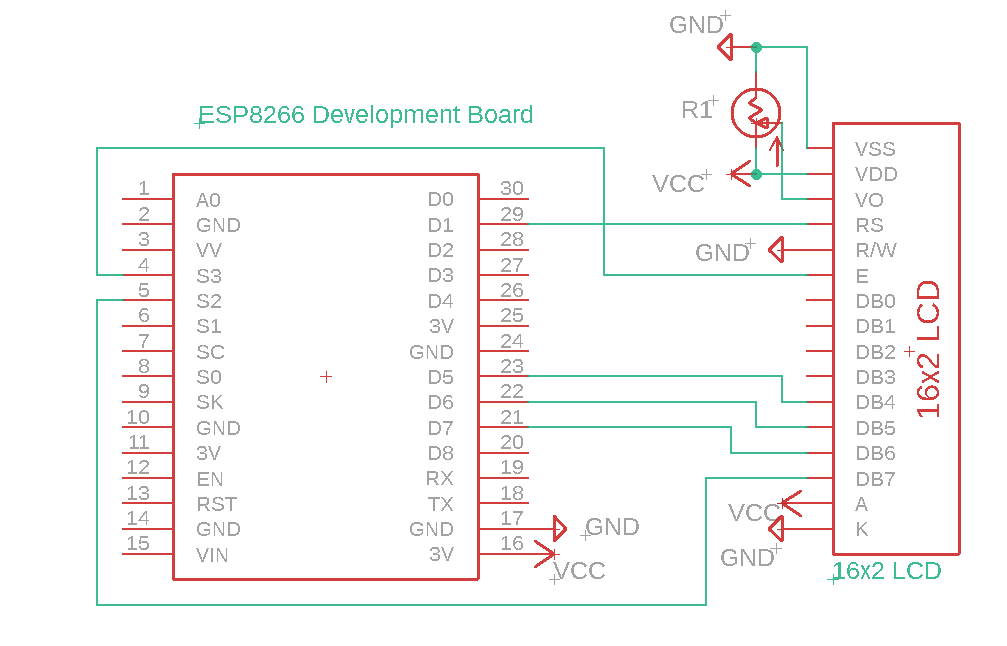
\includegraphics[max width=\textwidth,keepaspectratio,scale=.6]{images/ClientSchematic.png}
            \caption{\label{fig:ClientSchematic}Display schematic}
        \end{figure}

        The firmware was again made simple by the use of pre-made libraries.
        These libraries drove the Wi-Fi stack, and the 1602A LCD screen.

        The display firmware would first search for the Service Set Identifier (SSID) of a sensor unit.
        If it detects one, it would then connect and start requesting the weather at the rate of once a second.
        When the sensor reply came back, the display would then parse the incoming string and push the information to the LCD screen.

        The contrast of the display could be controlled by the potentiometer connected to the 1602A LCD display.

    \subsection{Further Development}
        In order to get a better demonstration of the capabilities of the project, 
        it was also possible for a computer to connect to the access point, and make a request of the sensor.
        To increase the human readability, the sensor would send a pre-defined webpage with the added environment values
        as seen in Figure~\ref{fig:Website}.

        \begin{figure}
            \centering
            \fbox{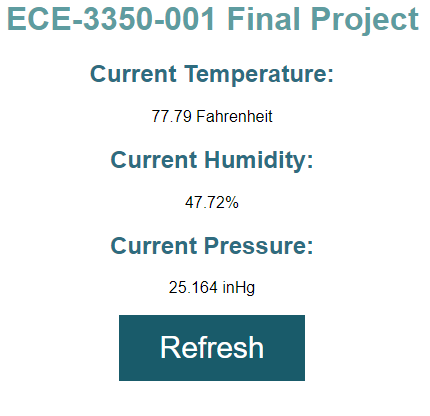
\includegraphics[max width=\textwidth,keepaspectratio,scale=.8]{images/Website.png}}
            \caption{\label{fig:Website}Human readable website transmitted by the sensor}
        \end{figure}

        Currently, only four devices can connect to the sensor access point at a time.
        This is due to limitations on the microcontroller.
        It is possible to get around this limitation by having the sensor connect to
        another Wi-Fi router, thereby offloading the requirement that it host the whole network traffic.

    \section{Results}
        As a whole, the project functions fairly reliably.
        The sensor and display will connect to each other, and if that connection is lost, will attempt to re-establish.

        With the current hardware, the maximum distance the two units were able to communicate with each other is forty three and a half feet.
        This distance was only achievable with direct line of sight between the two units.
        The final sensor unit can be seen in Figure~\ref{fig:SensorPhoto}, and the final display unit can be seen in Figure~\ref{fig:DisplayPhoto}.
        
        \begin{figure}
            \centering
            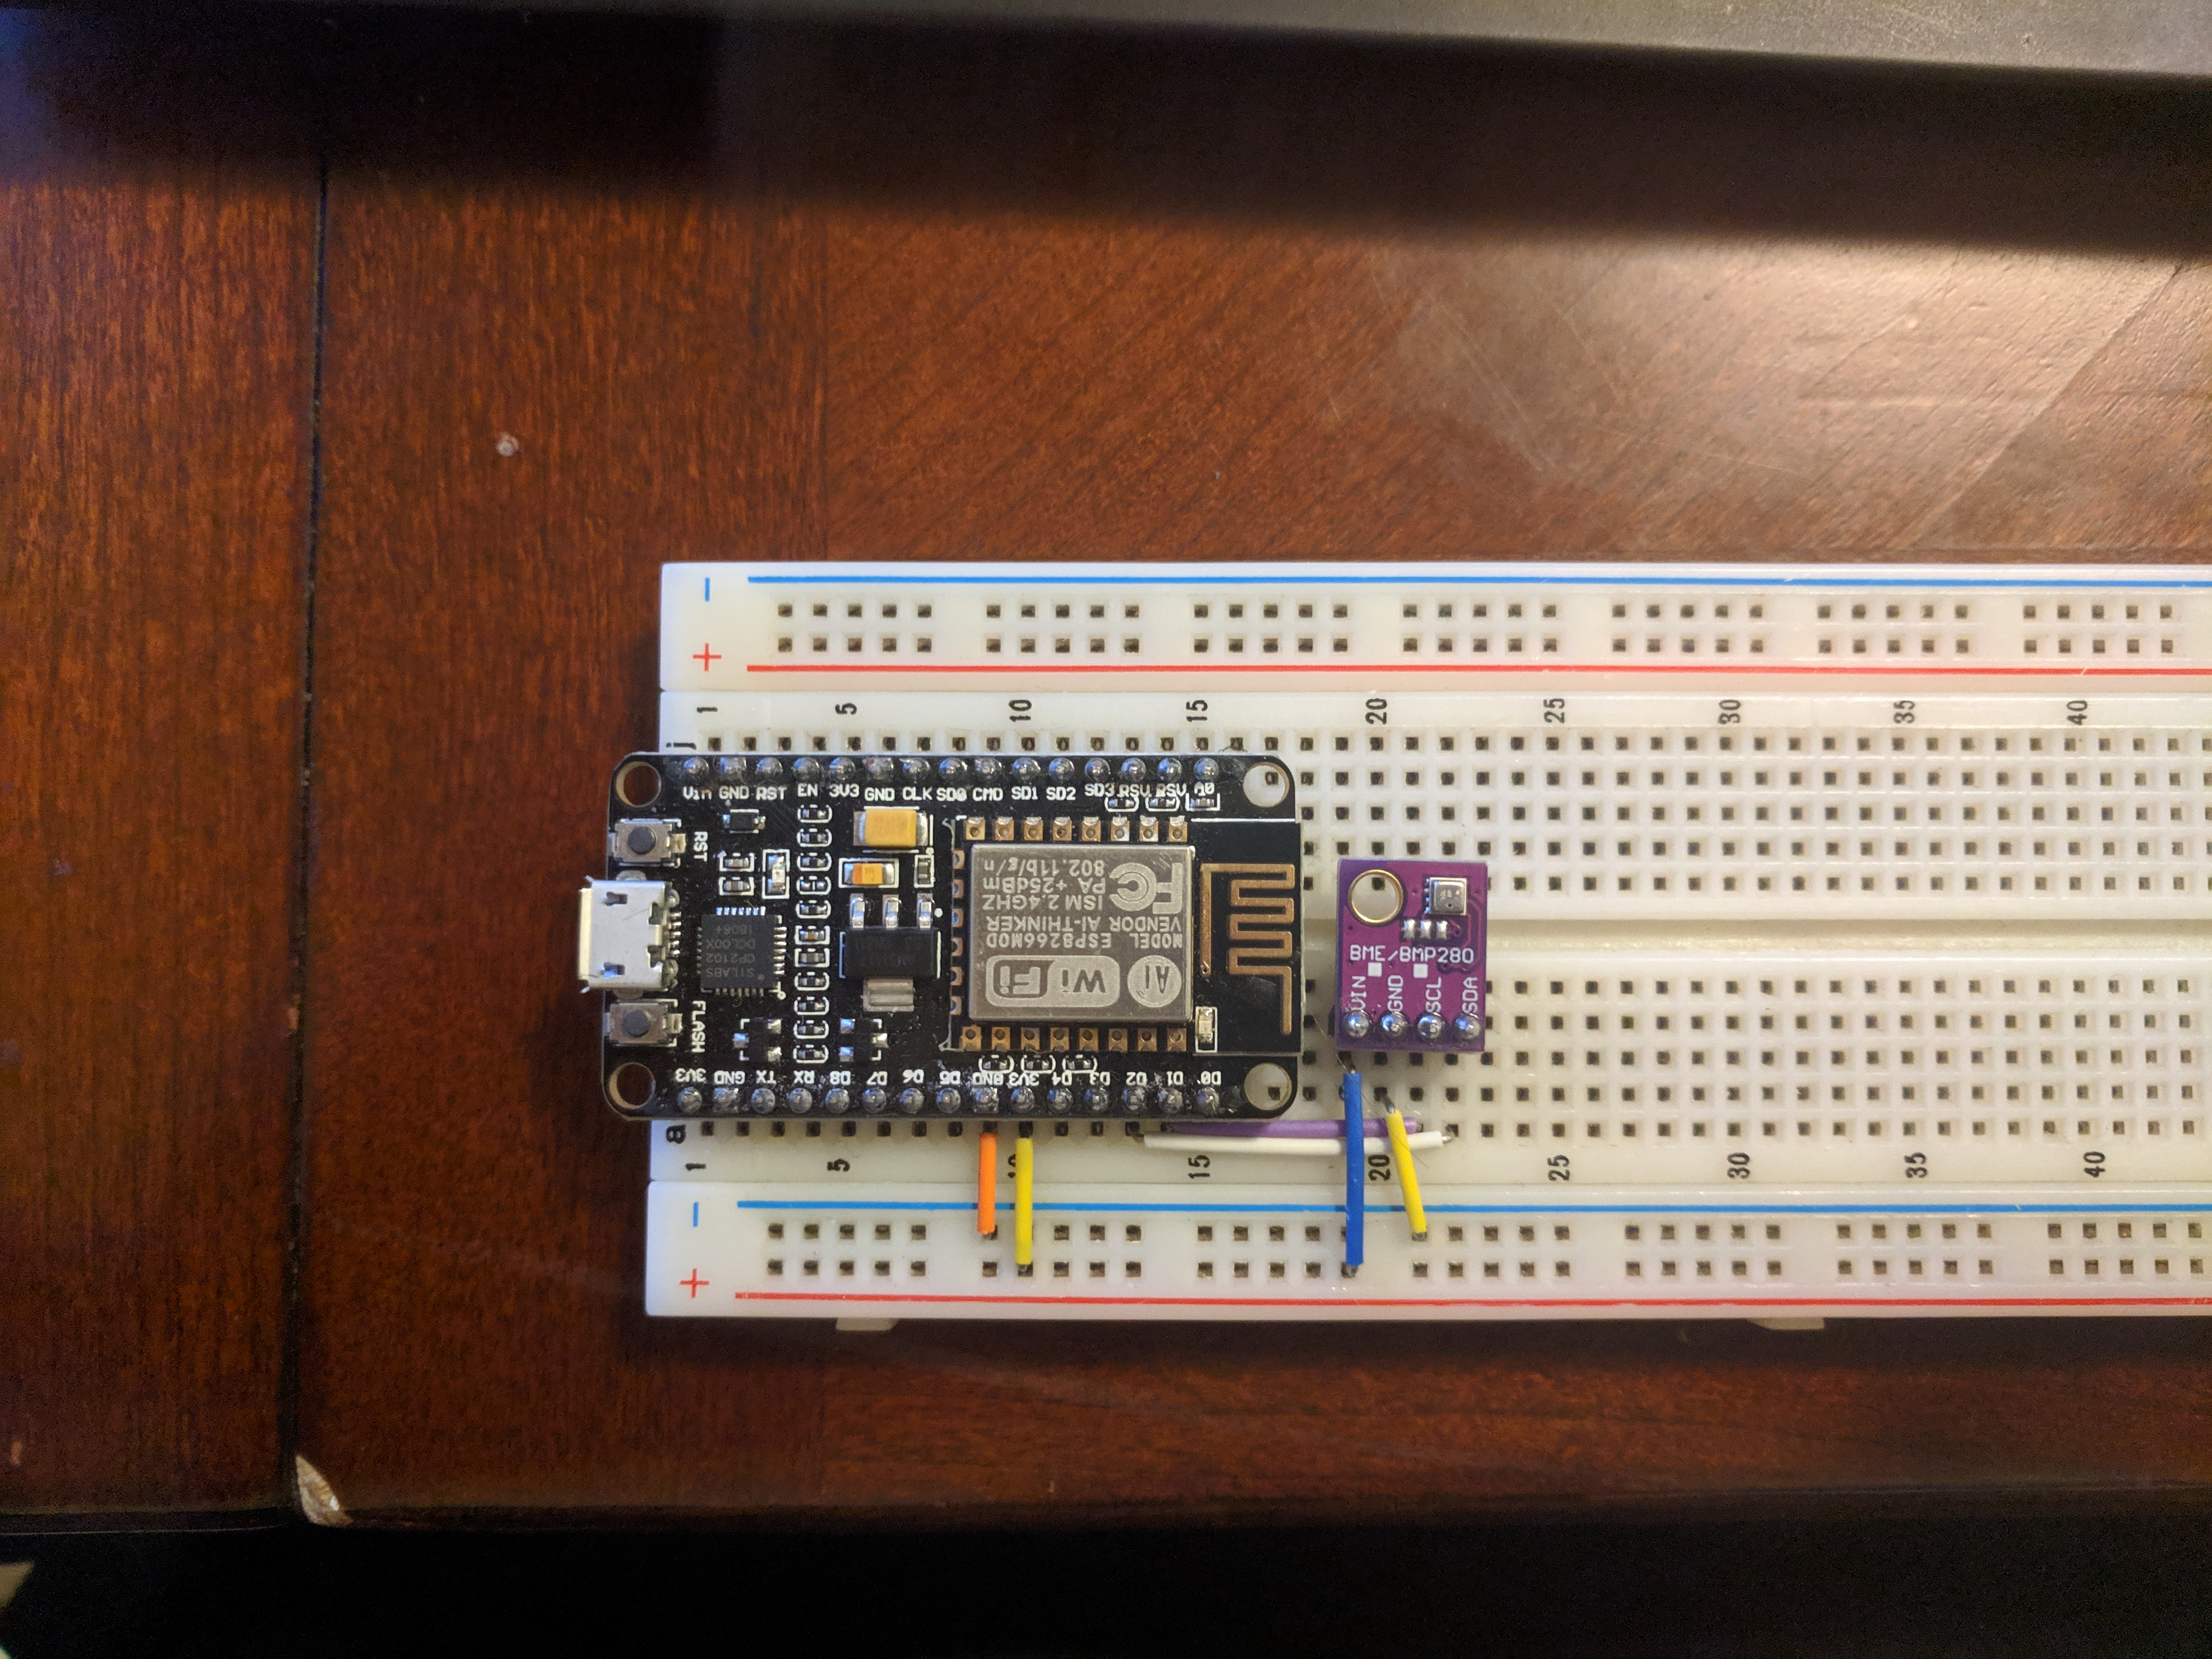
\includegraphics[max width=\textwidth,keepaspectratio,scale=.5]{images/ServerPhoto.jpg}
            \caption{\label{fig:SensorPhoto}Picture of the prototype sensor unit}
        \end{figure} 

        \begin{figure}
            \centering
            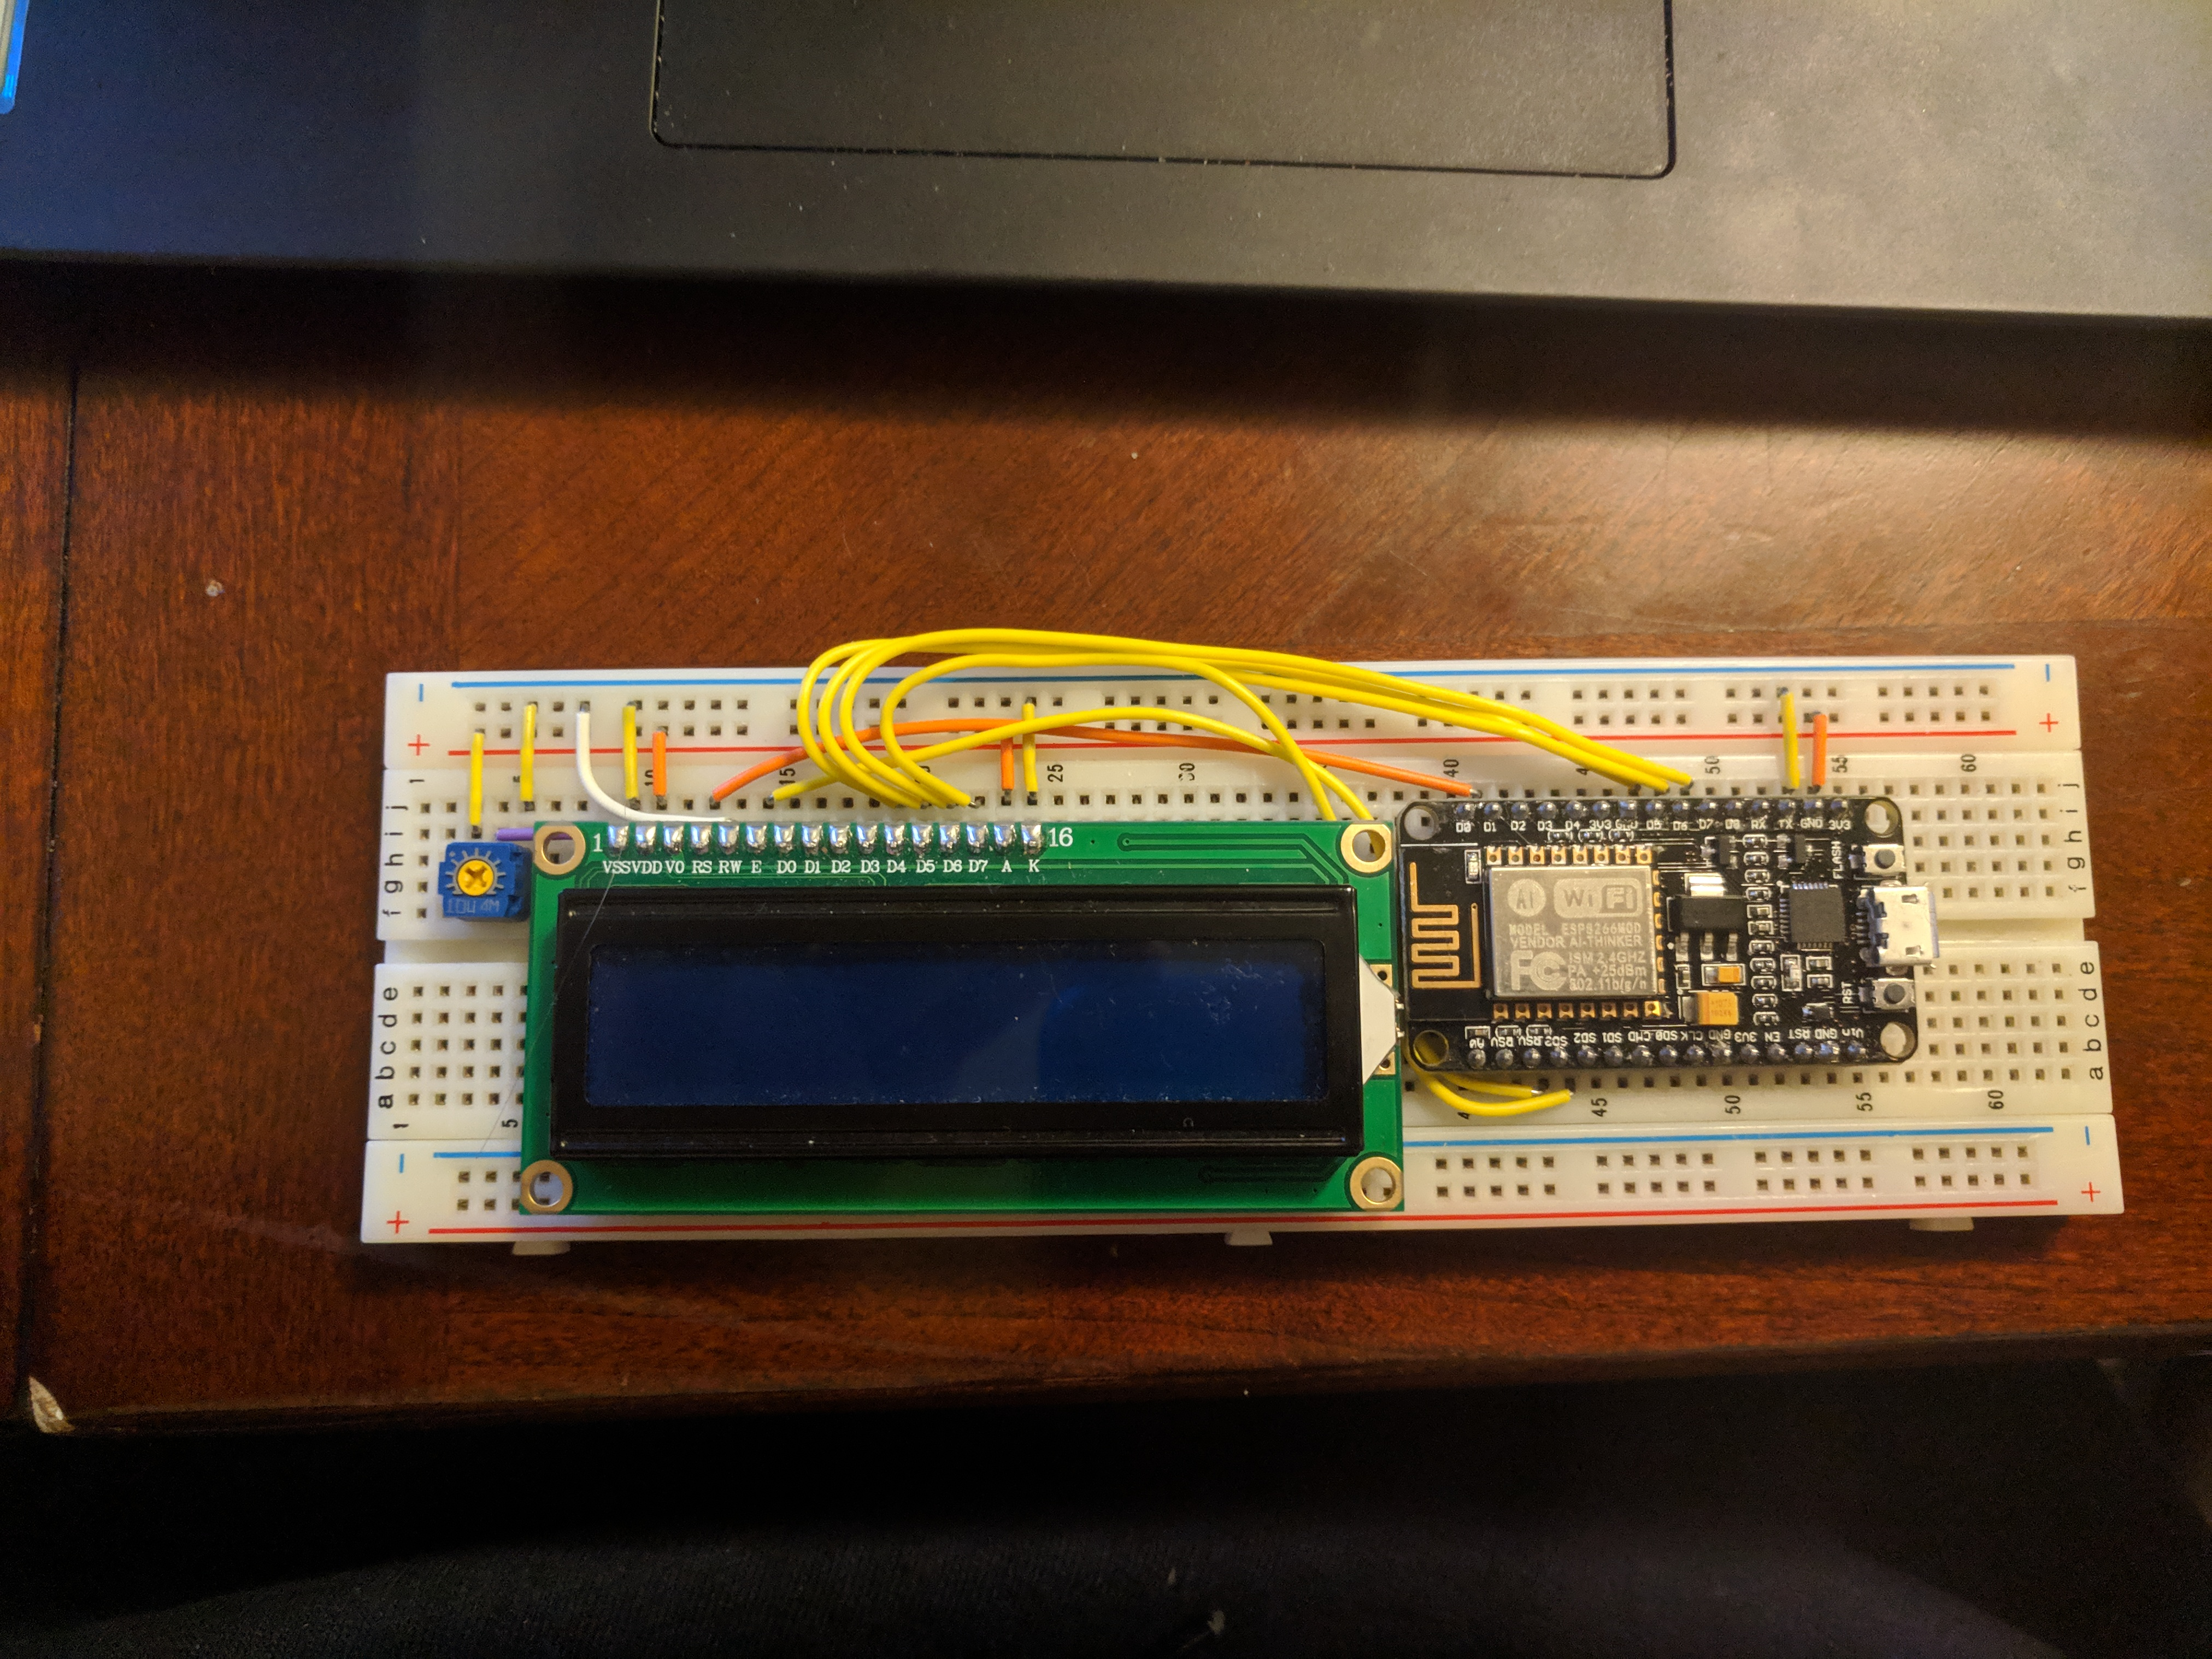
\includegraphics[max width=\textwidth,keepaspectratio,scale=.5]{images/ClientPhoto.jpg}
            \caption{\label{fig:DisplayPhoto}Picture of the prototype display unit}
        \end{figure}

    \section{Conclusion}
        This project was a fantastic foray into the world of Wi-Fi and IOT development.
        There are many tools that make the development of IOT devices fairly simple.
        The system is very robust for an initial look into having two or more devices communicate wirelessly.

        The improvements that can be made to the system include increasing the distance the sensor and display can communicate,
        pushing the sensor data to the cloud so that it can be accessed anywhere, adding more sensor types to the sensor, and many others.

    \bibliographystyle{IEEEConf}
    \bibliography{Bibliography.bib}
\end{document}